% Section name and highlighted ToC
%\renewcommand{\sectiontitle}{Introduction}
%\section{\sectiontitle}
%\customToC{currentsection,hideothersubsections}{}

% Section name and highlighted ToC
%\renewcommand{\subsectiontitle}{What is machine learning?}
%\subsection{\subsectiontitle}


\begin{frame}{Overview}
  \tableofcontents
\end{frame}
%%%% Work summary 


\begin{frame}{Spent time}
  From October 7th to 21st.  
  Total time around 20 hours. 
  \begin{figure}[t]
  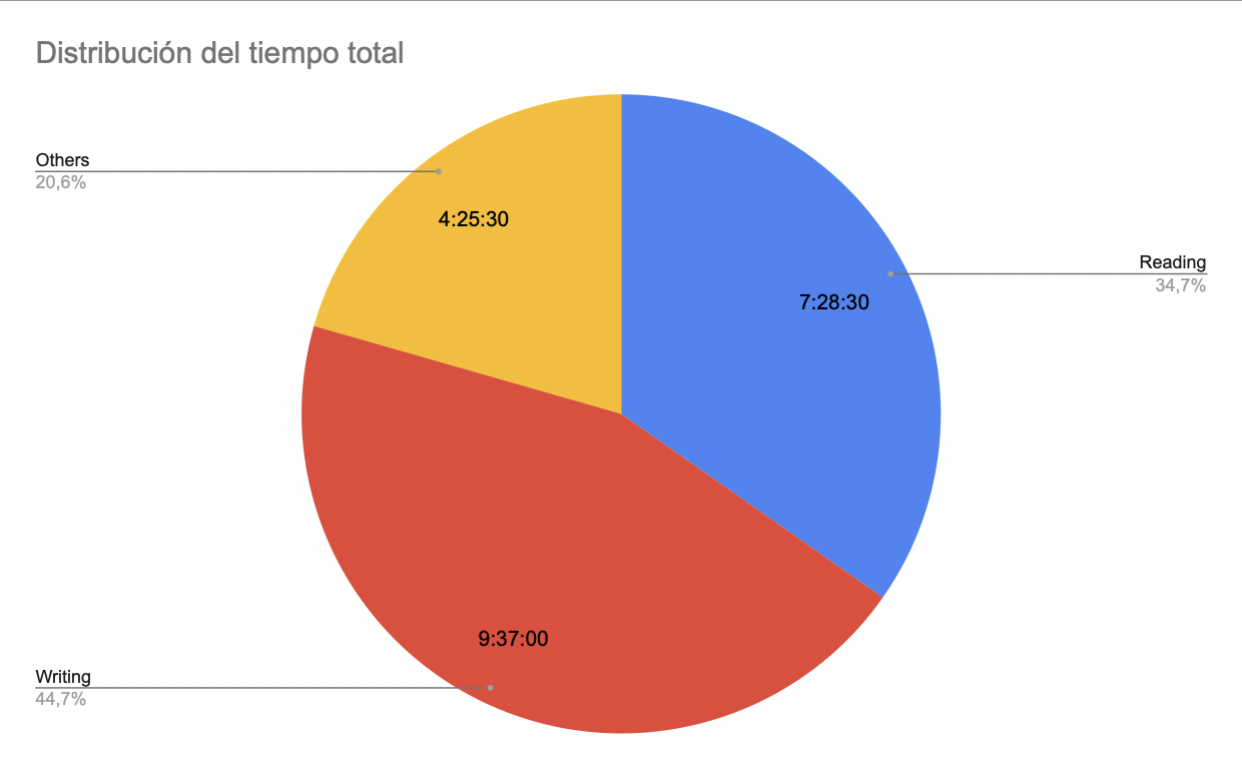
\includegraphics[height=0.7\textheight]{spent_times/october_21.png}
  \centering
  \end{figure}
\end{frame}
% Bishop definition of machine learning
\begin{frame}{Definition of machine learning}%{\subsectiontitle}
  \section{What is learning?}
    As it is said in the introduction of chapter one in  \cite{BishopPatternRecognition}
 \textbf{machine learning} \textit{is the field of pattern 
recognition that is concerned with the automatic
 discovery of regularities in data and the use of
these regularities to take actions such as 
classifying the data into different categories}.
\end{frame}

% --- Math formulation 
% 1. Naive perspective 
%\renewcommand{\subsectiontitle}{Math formulation}
%\customToC{currentsection,hideothersubsections}{}
%\subsection{\subsectiontitle}
\begin{frame}{Math formulation}
  \subsection{Math formulation}
    Let be
    \begin{itemize}
        \item an input vector $X \in \mathbb{R}^d$, 
        \item and out-put function $Y \in \mathbb{R}$.
    \end{itemize}
    
    \textbf{ 
      We seek a function $f(X)$ for predicting $Y$ given values of the input $X$.
      }
\end{frame}
% 2. Emphasized joint distribution
\begin{frame}{\textbf{My new} math formulation \footnote{ From \cite{HastieStatisticalLearing}}}
  
  Let be
    \begin{itemize}
        \item an input vector: $X \in \mathbb{R}^d$, 
        \item an out-put function: $Y \in \mathbb{R}$,
        \item  \textbf{with joint distribution $Pr(X,Y)$}.
    \end{itemize}
    
      We seek a function $f(X)$ for predicting $Y$ given values of the input $X$.

      \pause 
      \begin{theorem}{\textbf{The idealistic function}}  

      Exist a function $f: \mathbb{R}^d \longrightarrow \mathbb{R}$ that maps perfectly 
      every element of $(x,y) \in X \times Y$ ie 
      \begin{equation}
        \forall (x,y) \in X \times Y 
        \quad
        f(x) = y 
        \Longleftrightarrow
        P(y |X=x) = 1.
      \end{equation}
    \end{theorem} 
      \textbf{This is stricter than say they are $Pr(x,y)$ connected}.
    \end{frame}

    